\subsection{Flavor Tagging of Jets}
\label{sec:flavor_tagging}

The ability to identify jets containing heavy-flavored hadrons, i.e. jets containing
$b$- and $c$-flavored hadrons, is an important aspect to many of the most critical measurements
and analyses being done at the large LHC experiments.
The SM top-quark is the heaviest known elementary particle, the second-most recent elementary particle to be discovered,
and, given its importance to electroweak and Higgs physics, is an object subjected to high levels
of precise study at the LHC.
The top-quark decays before hadronisation timescales and therefore its decay products, which
are a $W$-boson and a $b$-quark nearly 100\% of the time, carry away information characterising its properties.
Being able to characterise the jets initiated by the hadronisation of these $b$-quarks, then,
is of critical import if the physics of the top-quark wish to be understood.
The recent discovery of an SM-like Higgs boson, with a mass of $m_h = 125\,\GeV$, decays
to a pair of $b$-quarks nearly 60\% of the time.
Without question, then, the thorough study of the Higgs boson necessitates the ability to precisely identify
the presence of the pair of $b$-initiated jets from its decays.
Additionally, we will see in subsequent chapters that the presence of $b$-quark initiated jets is
a characteristic signature of many BSM physics scenarios.
The identification of these types of jets, a process referred to as `flavor tagging', is of the utmost importance
to analyses performed with the ATLAS detector as well as in the work to be presented in this thesis.
Jets tagged as having likely arisen as a result of the hadronisation of an initiating $b$-($c$-)quark
are referred to as `$b$-tagged jets` (`$c$-tagged jets'), or simply as `$b$-jets` (`$c$-jets').
All other jets then are assumed to have arisen from the decay of light-flavor quarks and are referred to as `light-flavor jets' (`light-jets').

Heavy-flavor tagging of jets relies on the relatively long lifetimes of the $b$- and $c$-hadrons which
initiate them. The typical $b$-hadron lifetime is $\tau \approx 1.6$\,ps ($c\tau \approx 450\,\micron$),
which leads to $b$-hadrons traversing typically macroscopic distances away from the primary hard-scatter vertex
before they decay.
As seen in Figure~\ref{fig:bhadron_decay_length}, $b$-hadrons with transverse momenta on the order of
$50\,\GeV$ will travel nearly half a centimeter before decaying.
Also seen in Figure~\ref{fig:bhadron_decay_length}, those $b$-hadrons with \pT~values nearing $250\,\GeV$ will actually decay
outside of the beam-pipe within the region of the IBL.
Given the high spatial resolution of the ID pixel and SCT detectors discussed in Section~\ref{sec:inner_detector}, the presence of these long-lived particles
should be detectable via the presence of at least one secondary decay vertex corresponding to the point at which
the heavy-flavored hadron decays.
Figure~\ref{fig:bjet_decay} illustrates the standard topology of a heavy-flavor initiated jet with a secondary decay vertex that is displaced
with respect to the primary hard-scatter vertex and is the source of displaced tracks.

The algorithms used to identify heavy-flavor initiated jets, then, rely on information characterising
the long lifetimes of the initiating particles and on the presence of secondary decay vertices within the jet.
These high-level algorithms used to identify these jets take as input information provided by taggers that rely on low-level information based on
the presence of displaced tracks and secondary vertices.
These low-level taggers will be introduced in Section~\ref{sec:ftag_low_level} and the construction of the
high-level tagger, used in the analyses to be presented in this thesis, will be presented in Section~\ref{sec:ftag_high_level}.


%%%%%

%As in Ref.~\cite{ATL-PHYS-PUB-2017-013}.


\begin{figure}[!htb]
    \begin{center}
        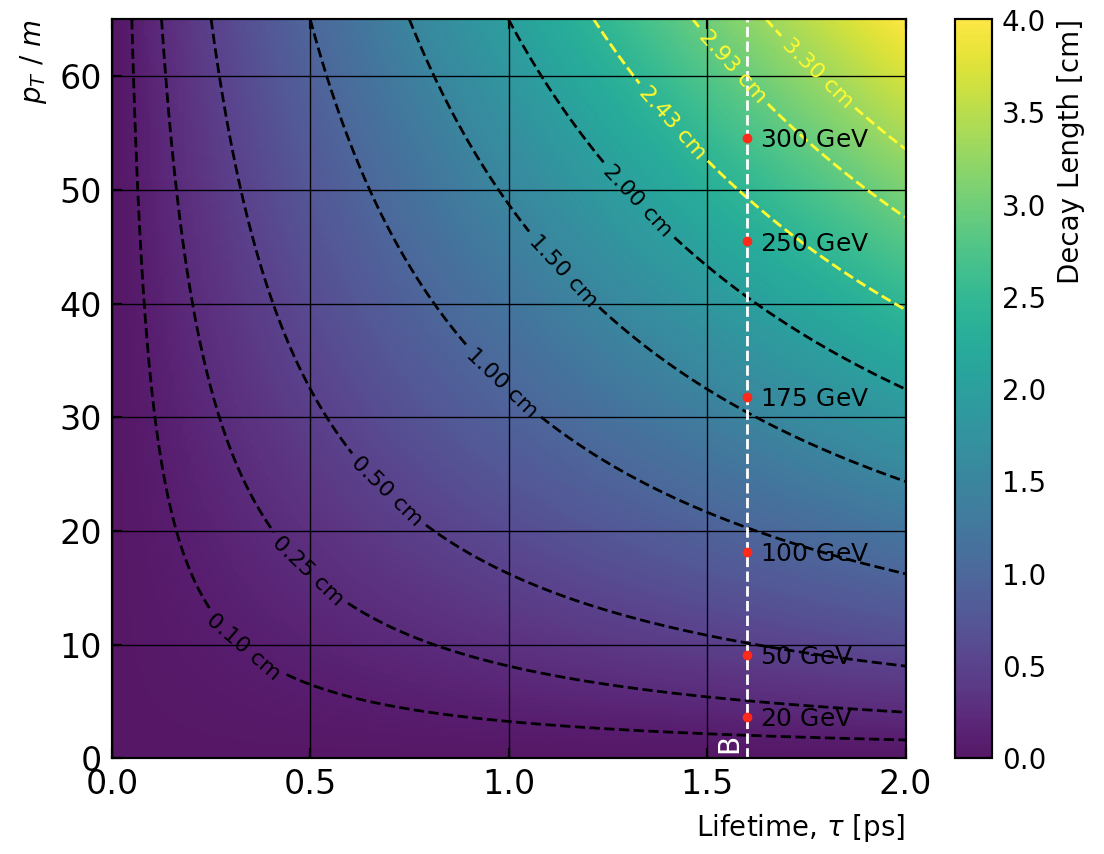
\includegraphics[width=0.7\textwidth]{figures/bhadron_decay_length_ibl}
        \caption{
            Particle decay length as a function of its lifetime and transverse momentum normalised
            to its rest mass.
            The white-dashed line indicates the average lifetime of $B$-hadron species, taken
            as 1.6\,ps, with a mass taken to be 5.5\,GeV.
            The red-dots along the $B$-hadron line indicate locations for specific transverse momenta
            for the decaying $B$-hadron.
            The yellow contours indicate the locations of the IBL (Figure~\ref{fig:pixel_detector_trans}),
            with 2.43\,cm corresponding to the beam-pipe radius.
            {\color{red}{Perhaps move this plot elsewhere?}}
            {\color{red}{Add references to PDG}}
        }
        \label{fig:bhadron_decay_length}
    \end{center}
\end{figure}

\begin{figure}[!htb]
    \begin{center}
        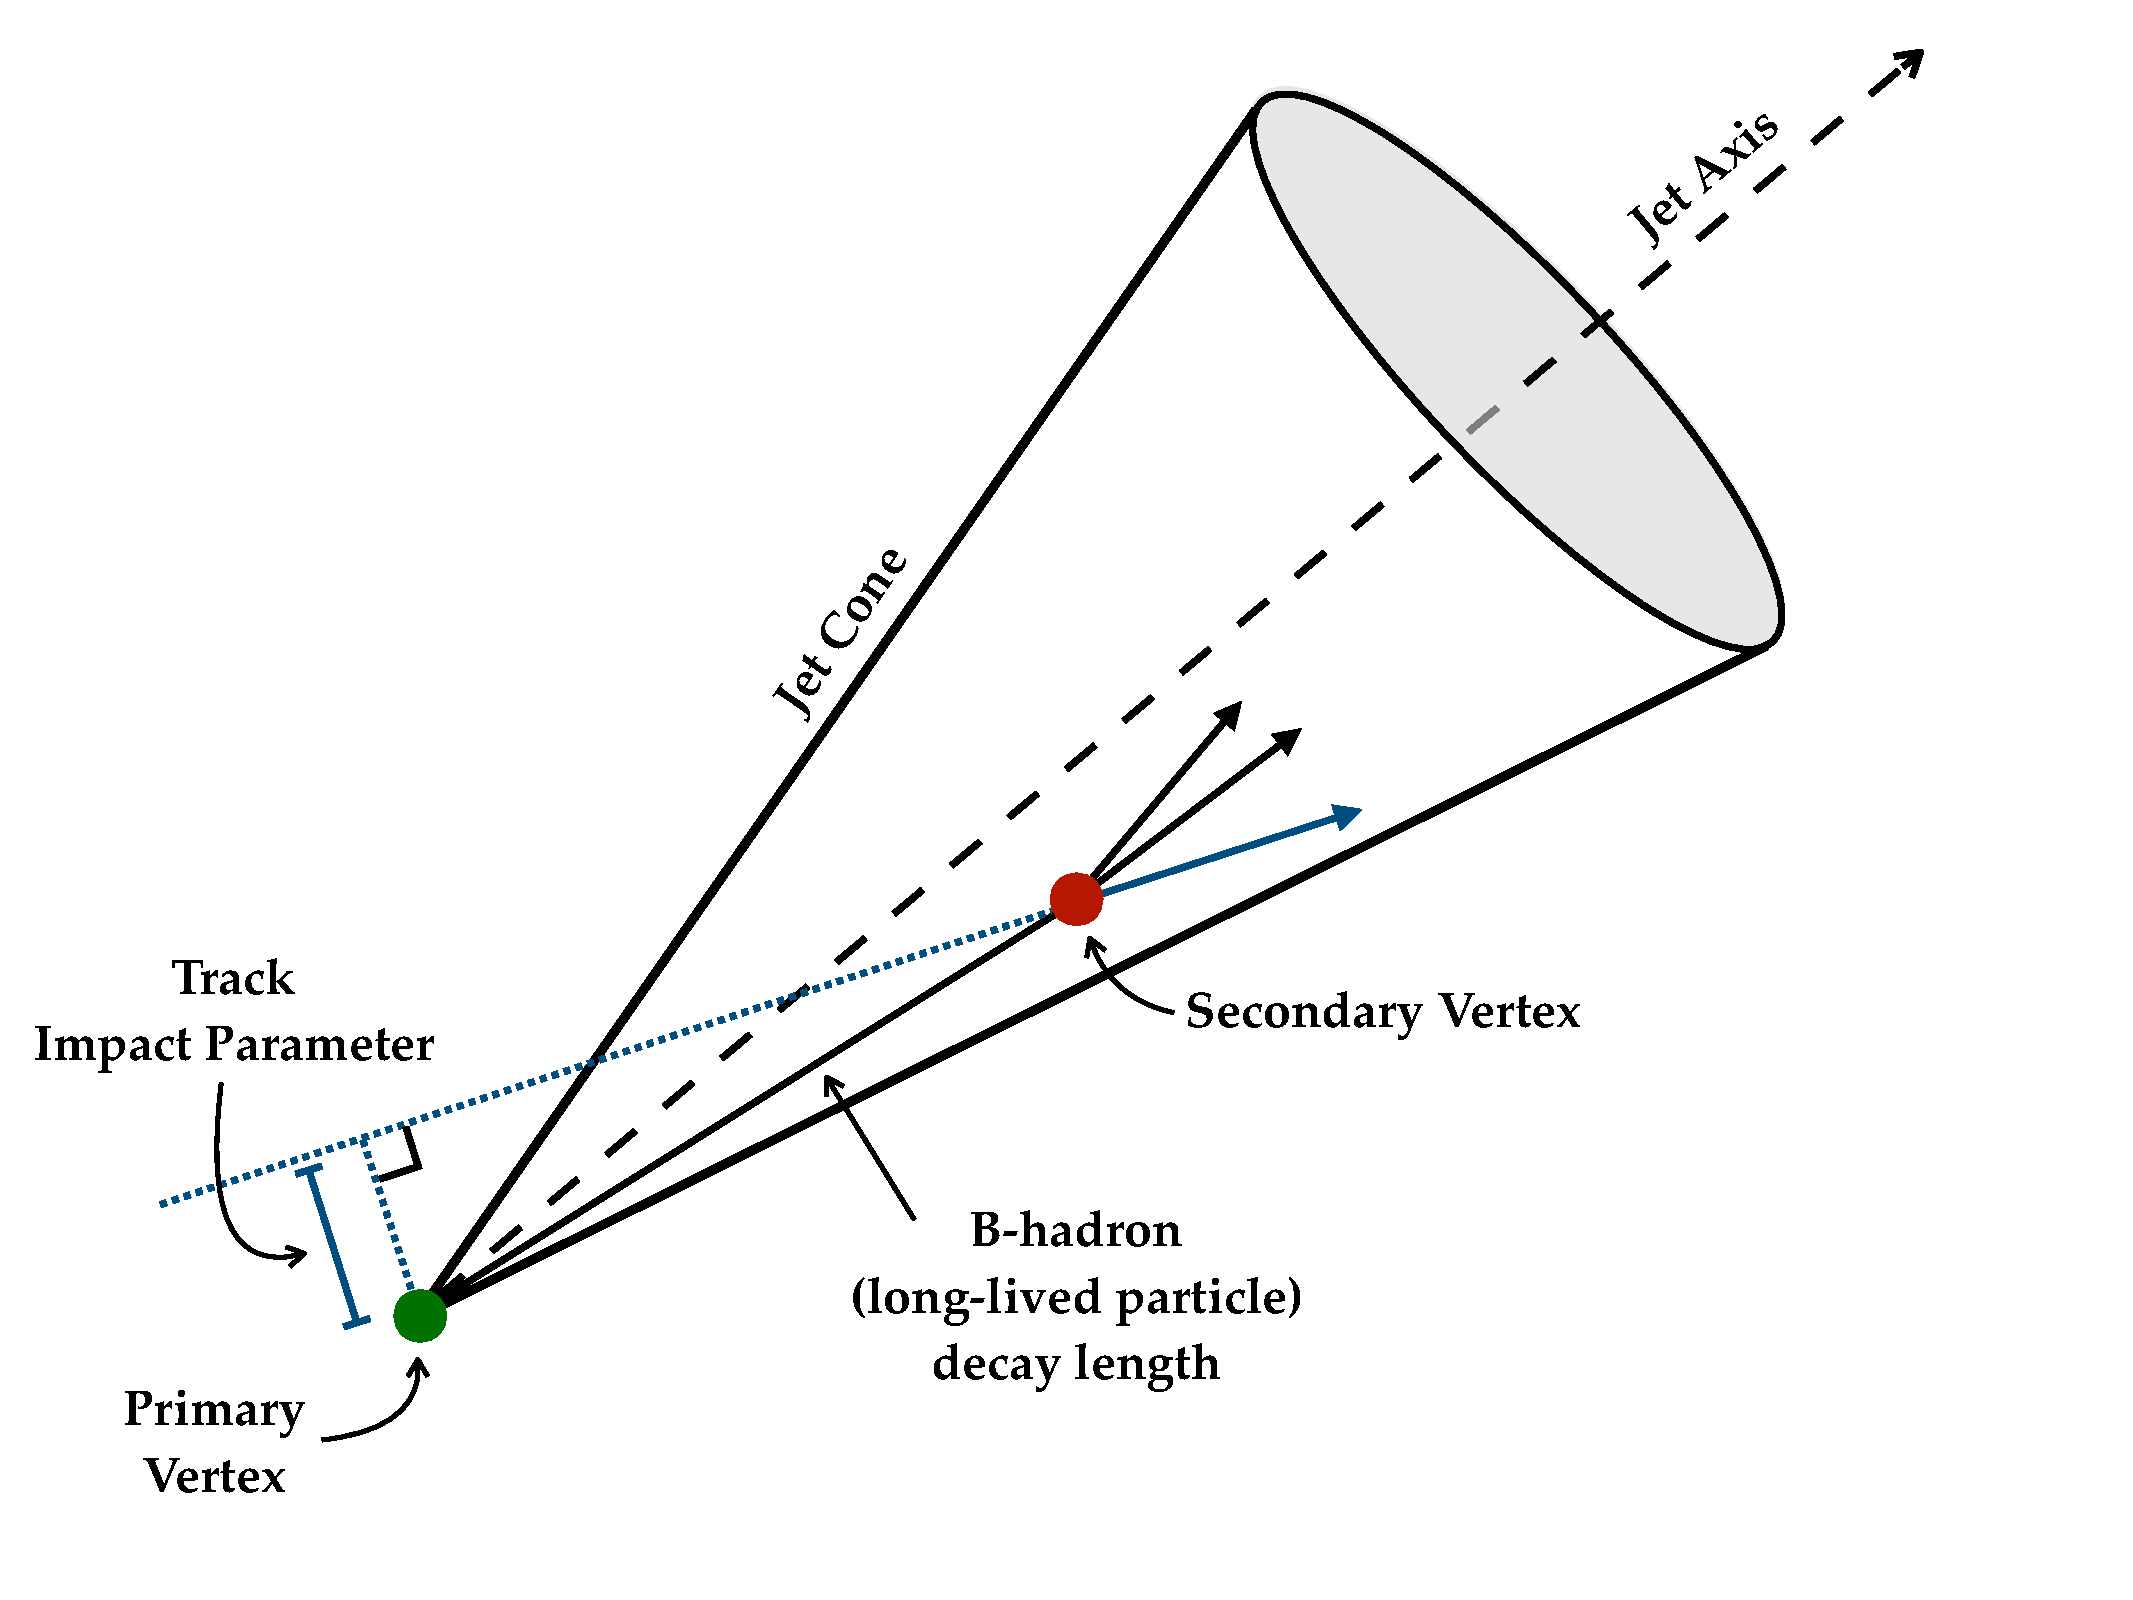
\includegraphics[width=0.7\textwidth]{figures/chapter3/ftag/bhadron_decayPDF}
        \caption{
            Topology of a $b$-jet.
            The $b$-hadron produced near the primary hard-scatter vertex (green dot), initiating the
            $b$-jet, has a long lifetime and decays a macroscopic distance away from the primary
            hard-scatter vertex to produce a secondary vertex (red dot) from which additional tracks
            are produced and subsequently reconstructed.
            The tracks originating from the secondary vertex will have larger impact parameters relative
            to the primary hard-scatter vertex as compared to tracks originating from the primary
            hard-scatter vertex.
        }
        \label{fig:bjet_decay}
    \end{center}
\end{figure}

%\FloatBarrier
\subsubsection{Low Level Taggers and Inputs}
\label{sec:ftag_low_level}

The final algorithm used to identifiy $b$-tagged jets take as input the outputs from several low-level
$b$-tagging algorithms.
There are two classes of low-level algorithms: those that rely on the impact parameter information of the
tracks associated with the jets and those that rely on the explicit reconstruction of secondary decay vertices
within the jet~\cite{FTAG2019}:

\begin{itemize}
    \item{\textbf{IP2D and IP3D}} The IP2D and IP3D algorithms make use of the signed transverse impact parameter significance of tracks
        to construct discriminating variables. The IP3D algorithm additionally makes use of the longitudinal impact parameter
        significance. The algorithms rely on constructing log-likelihood ratios (LLR) taking as inputs probability density functions (PDFs)
        for $b$-, $c-$, and light-flavor jet probabilities on a per-track basis.
    \item{\textbf{Secondary Vertex Finding Algorithm (SV1)}} The SV1 algorithm~\cite{SV1} reconstructs a single displaced secondary vertex within
        a jet, starting from the set of all possible two-track vertices while rejecting tracks likely to be associated with
        non-heavy-flavored long-lived particles ($K_s$ or $\Lambda$), photon conversions, or vertices due to detector material interactions.
        The inclusive secondary vertex and associated tracks are then used to construct discriminating observables sensitive to the differences
        between $b$-, $c$-, and light-flavor jets.
    \item{\textbf{Multi-vertex Finding Algorithm (JetFitter, JF)}} The JetFitter algorithm~\cite{JETFITTER} attempts to reconstruct the full
        $b$-hadron decay chain using a modified Kalman filter~\cite{KalmanFilter} which assumes a common line on which the primary, $b$-hadron,
        and $c$-hadron decay vertices lie. As with SV1, the construction of many discriminating observables related to the
        reconstructed set of vertices are used to build templates for $b$-, $c$-, and light-flavor jets.
\end{itemize}

Figure~\ref{fig:ftag_low_level_var} provides an example of a few observables provided by the low-level tagging algorithms.

\begin{figure}[!htb]
    \begin{center}
        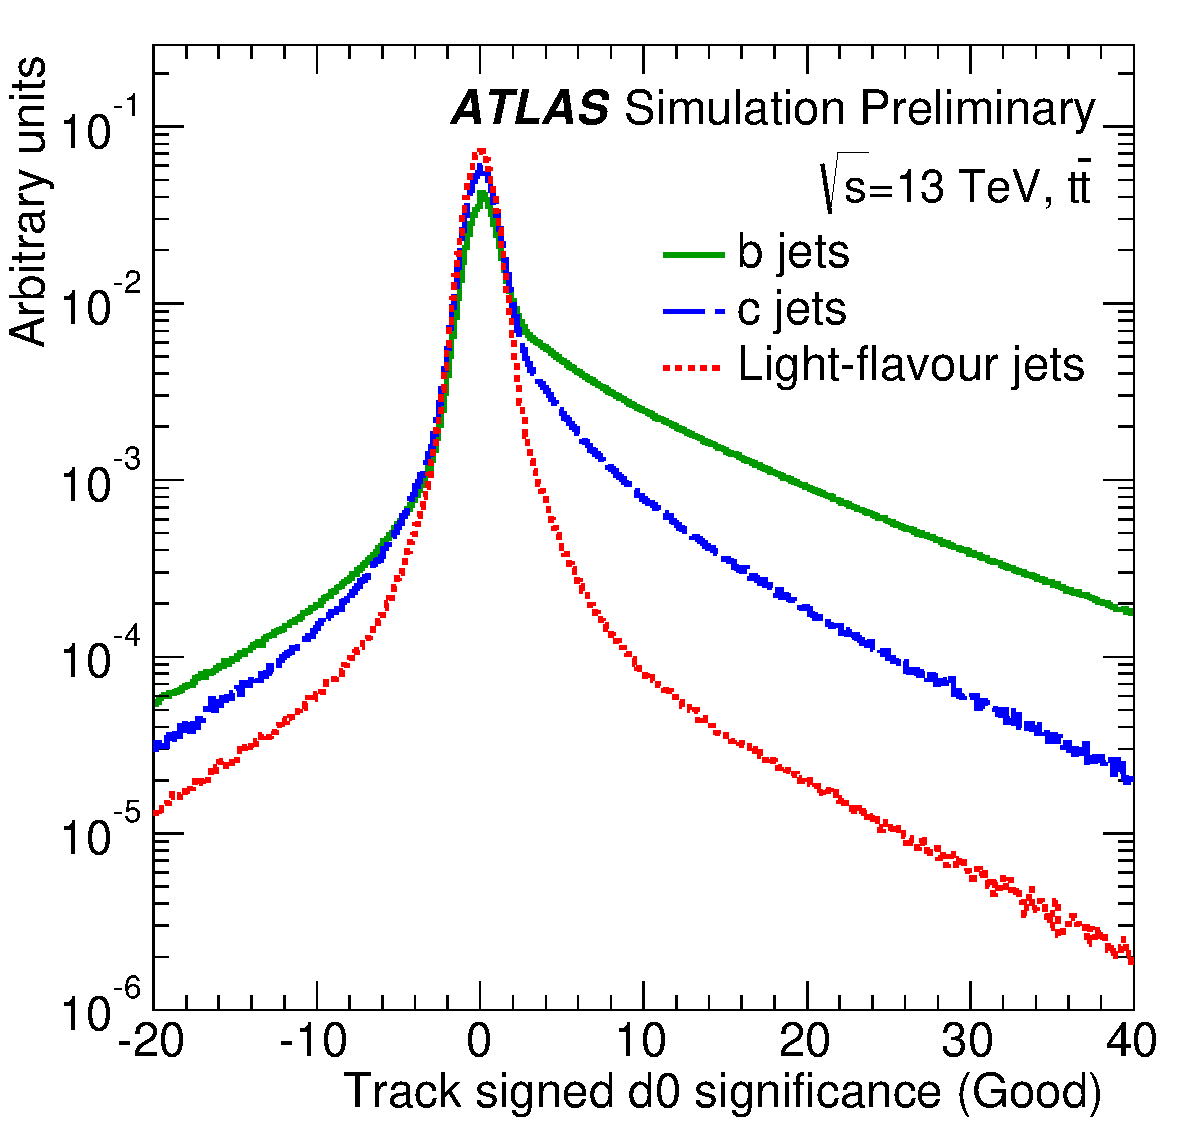
\includegraphics[width=0.32\textwidth]{figures/chapter3/ftag/ftag_track_d0_sig_ip2d}
        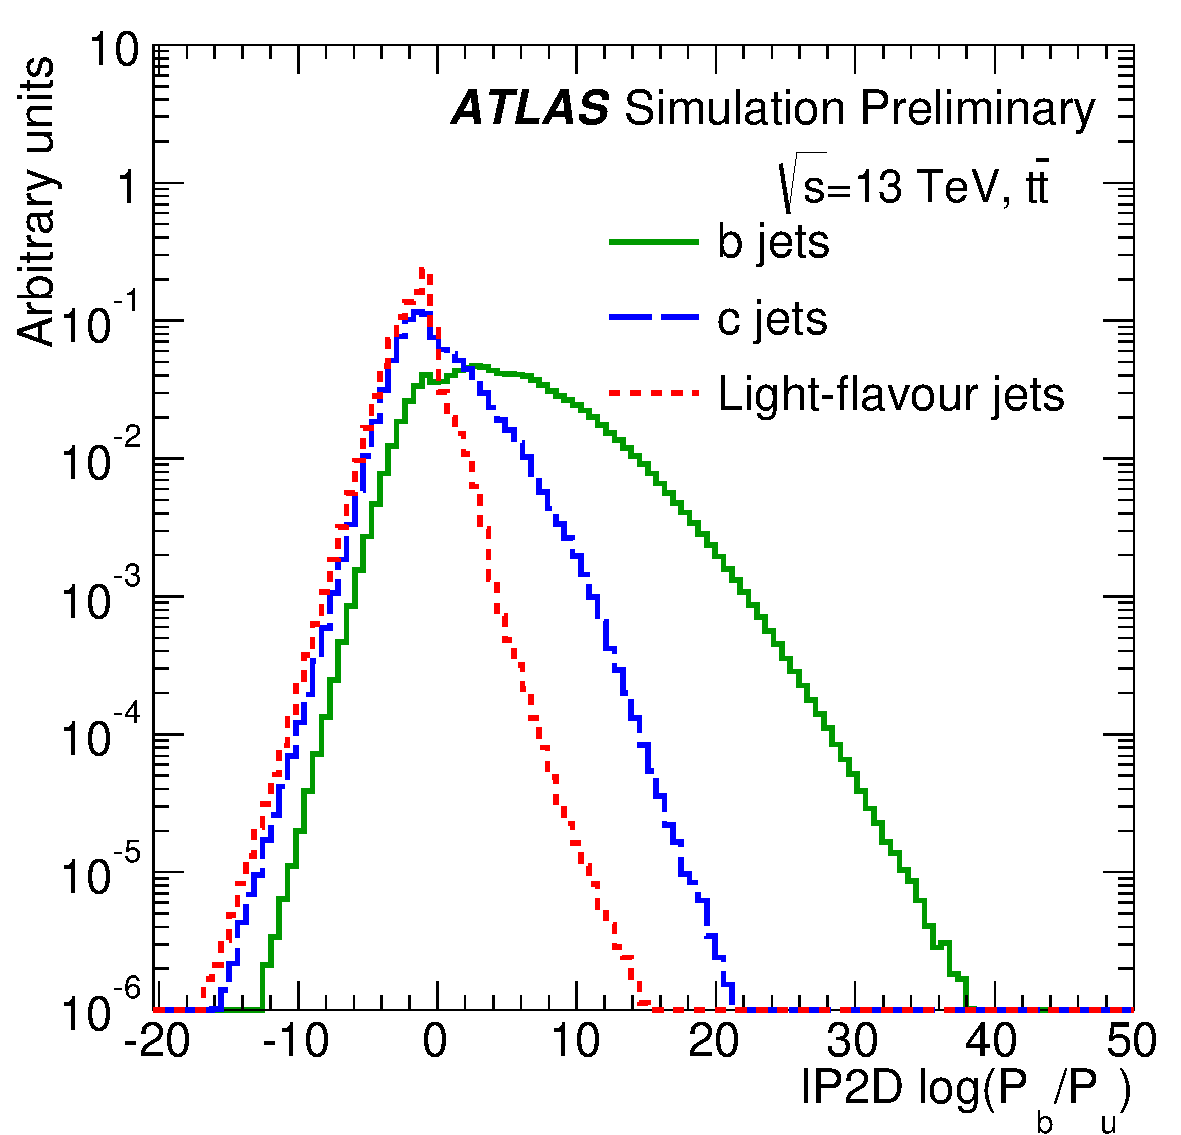
\includegraphics[width=0.32\textwidth]{figures/chapter3/ftag/ftag_ip2d_pb}
        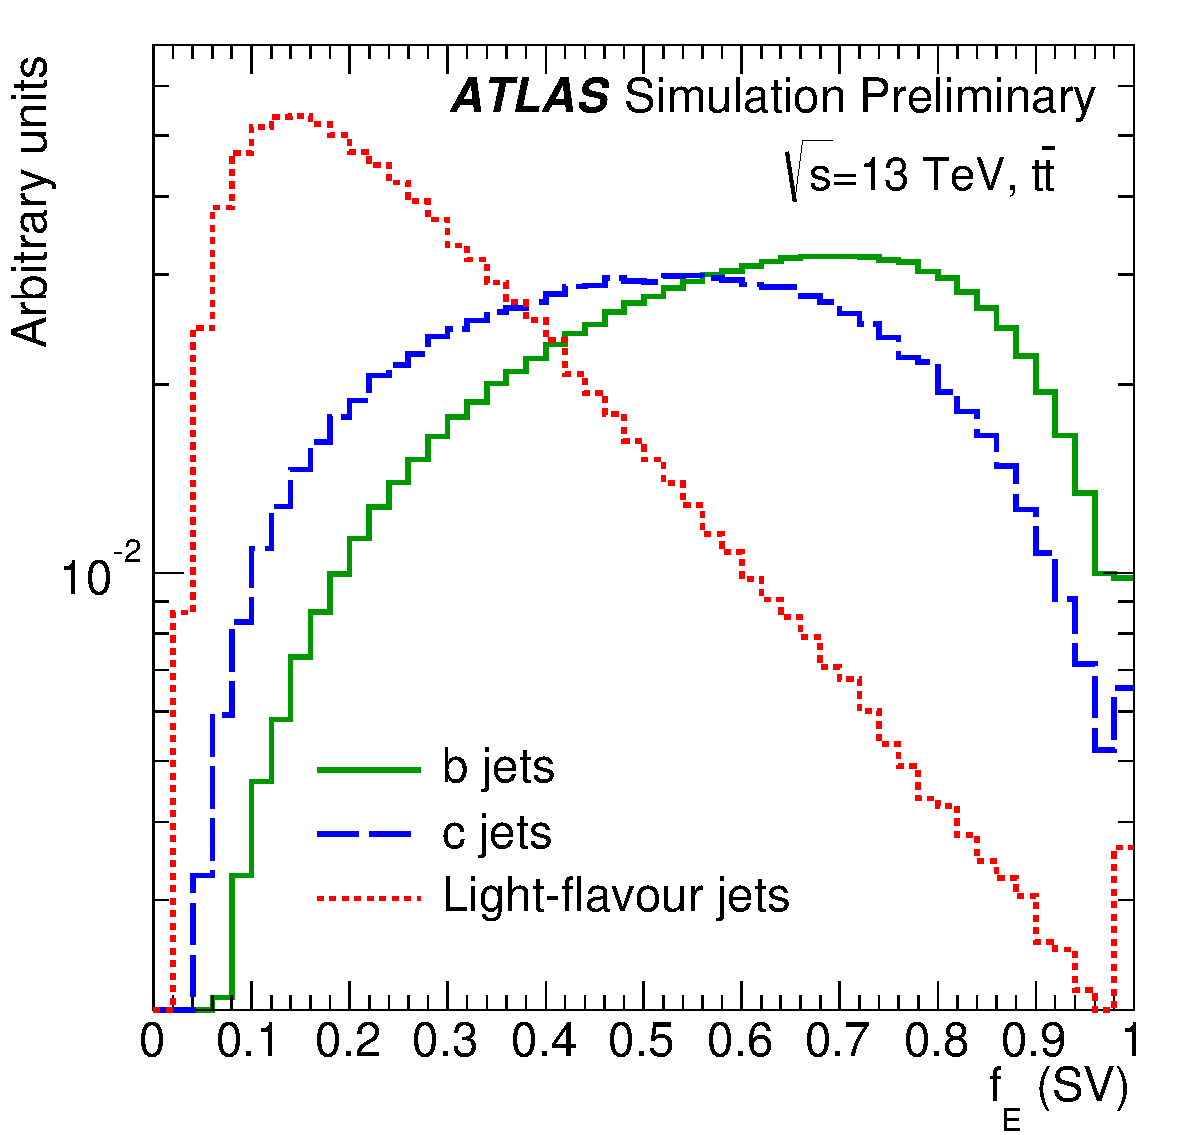
\includegraphics[width=0.32\textwidth]{figures/chapter3/ftag/ftag_sv1_fE}
        \caption{
            Examples of a few low-level quantities used in the ATLAS flavor tagging algorithms.
            The blue histograms are distributions associated with $b$-jets, green are those of $c$-jets, and red
            are those of light-flavor jets.
            \textit{Left}: Two-dimensional (signed) $d_0$ significance for tracks matched to jets.
            \textit{Middle}: IP2D $b$-jet log-likelihood ratio.
            \textit{Right}: Energy fraction, defined as the energy of the tracks in the displaced
                vertex reconstructed by the SV1 algorithm relative to the energy of all tracks in the jet.
%            Figures taken from Ref.~\ref{ATL-PHYS-PUB-2016-022}.
        }
        \label{fig:ftag_low_level_var}
    \end{center}
\end{figure}

%\FloatBarrier
\subsubsection{High Level Tagger: MV2}
\label{sec:ftag_high_level}

The low-level taggers discussed in the previous section provide a set of many useful and complementary observables.
In an attempt to make the most efficient use of all the information provided by this set of observables,
a boosted decision tree (BDT) algorithm is used to combine the outputs of these low-level algorithms.
This algorithm, referred to as the MV2 $b$-tagging algorithm, is trained using the ROOT Toolkit for Multivariate
Data Analysis (TMVA)~\cite{TMVA}.
In the analyses based on data recorded by ATLAS between 2015--2016, the MV2 algorithm was trained using jets from
a simulated sample of top-quark pair production events.
For the analyses based on the full Run-II data recorded by ATLAS, up to and including the year 2018, the MV2
algorithm was retrained using a sample composed of jets both from top-quark
pair production events as well as from simulated events of a BSM physics scenario of a heavy $Z^{\prime}$ decaying to $b\bar{b}$.
The latter was included in the retraining so as to allow the algorithm to have in its training sample
high-\pT~jets that are not present in the SM top-quark pair production events, as illustrated in Figure~\ref{fig:ftag_mv2c10_disc}.

Figure~\ref{fig:ftag_mv2c10_disc} shows a distribution of the MV2 algorithm's output.
The MV2 score is computed on a per-jet basis, using the set of low-level inputs listed in Table~\ref{tab:ftag_mv2_inputs}.
Working points, defined with different target-efficiencies for accepting $b$-tagged jets, are defined
by selection thresholds on the MV2 discriminant.
The standard ATLAS $b$-tagging working points are defined for accepting $b$-jets with $\pT>20\,\GeV$ with
average efficiencies of 60\%, 70\%, 77\%, and 85\%. 
The working points are based on selections made on the MV2 output score and are defined in Table~\ref{tab:btag_wp}, along with the rejection factors\footnote{The rejection factor
is defined as the inverse of the efficiency. A rejection factor of 100 means, therefore, that the associated
object is accepted --- on average --- 1 out of every 100 times that it appears.}
for $c$-jets, $\tau$-jets\footnote{Hadronically decaying $\tau$ leptons are accepted by the $b$-tagging algorithms
at rates higher than light-flavor jets due to the non-negligible decay length of the $\tau$ lepton which give them $b$-like
characteristics.},
and light-flavor jets.



\begin{figure}[!htb]
    \begin{center}
        \raisebox{1.5cm}{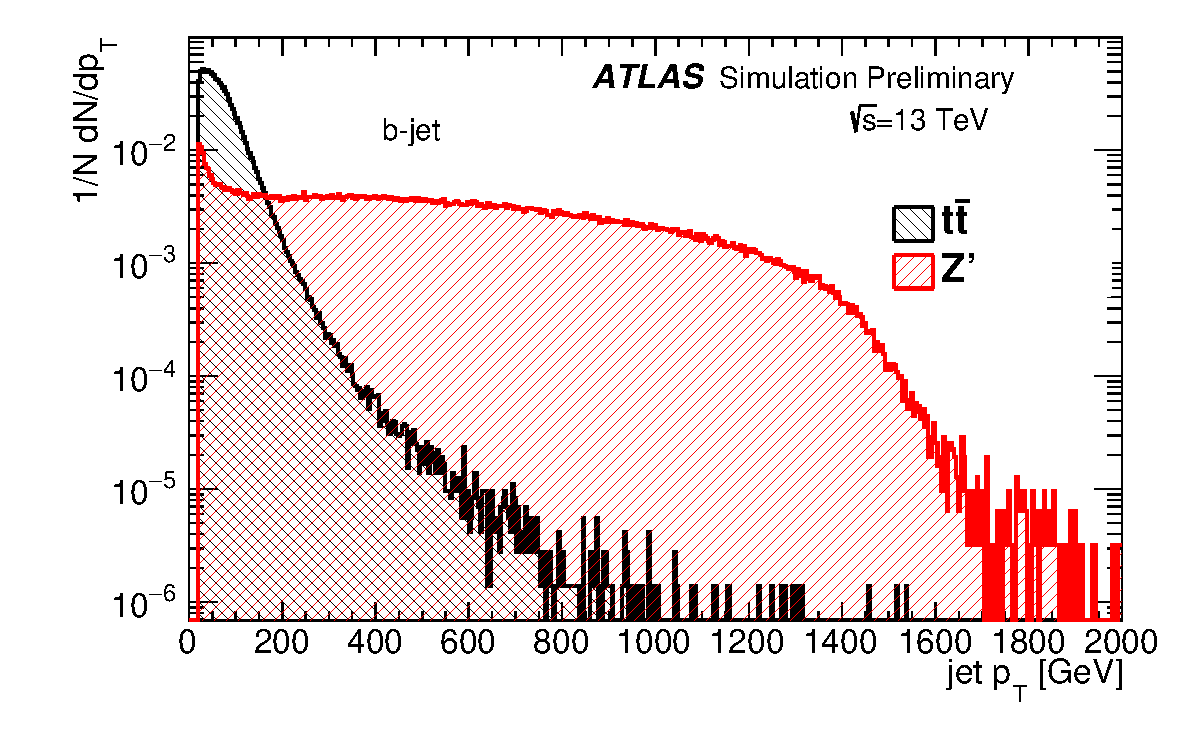
\includegraphics[width=0.48\textwidth]{figures/chapter3/ftag/ftag_train_sample}}
        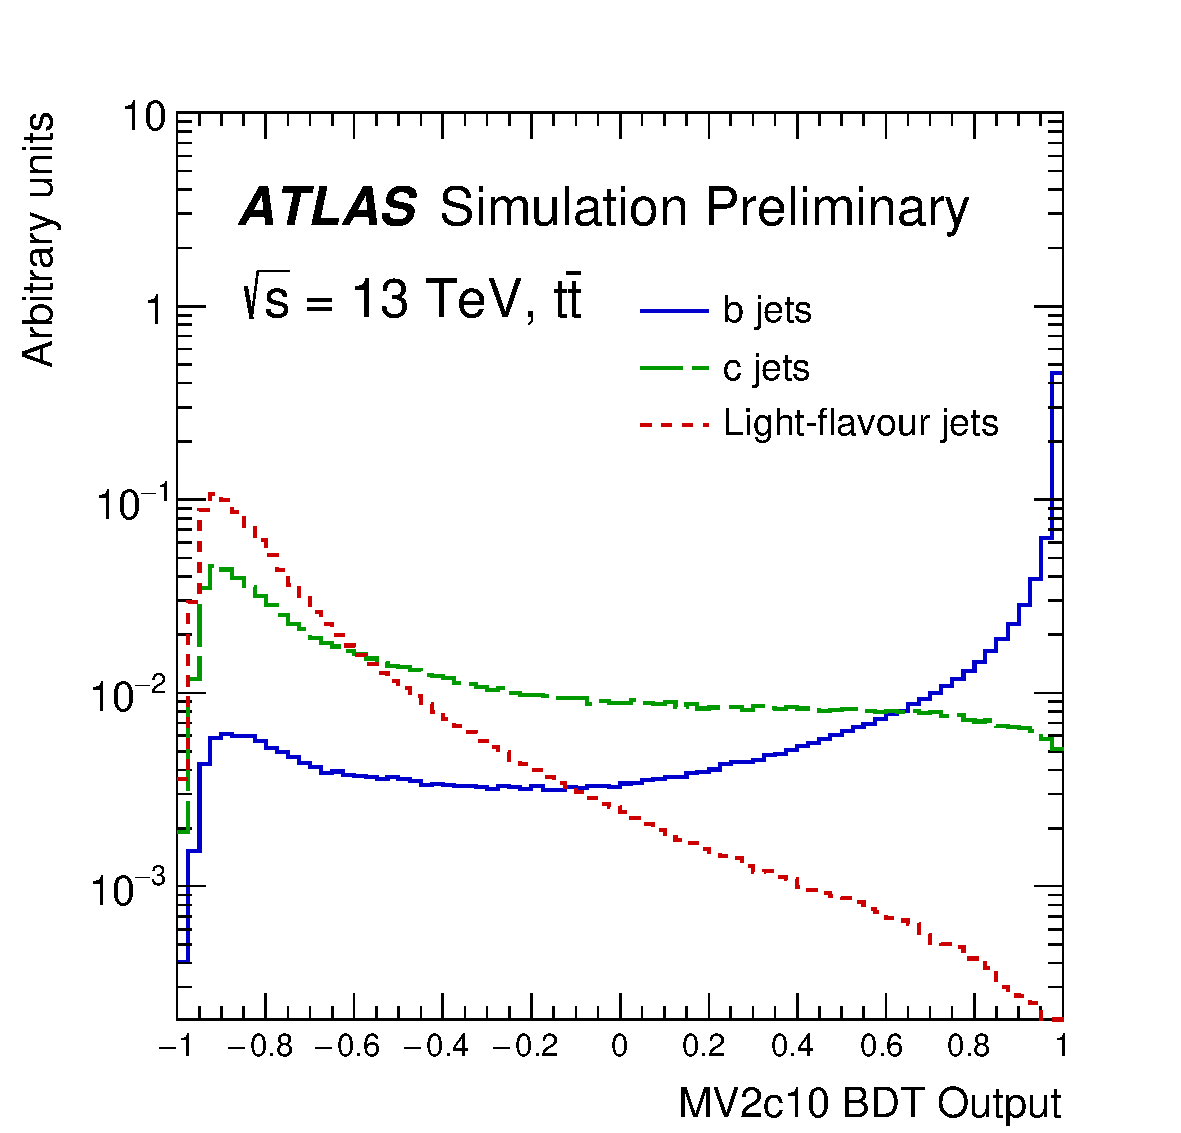
\includegraphics[width=0.48\textwidth]{figures/chapter3/ftag/ftag_mv2c10_disc}
        \caption{
            \textit{Left}: Distribution of jet \pT~for jets used in the training of the MV2 BDT algorithm.
                The $Z^{\prime}$ sample of jets is only included in the MV2 training relevant to the analyses
                based on the full Run-II dataset collected by ATLAS.
            \textit{Right}: Distribution of the BDT-based MV2 $b$-tagging algorithm output score, shown for
                $b$-jets (blue), $c$-jets (green), and light-flavor jets (red).
%            Figures taken from Ref.~\ref{ATL-PHYS-PUB-2016-012}.
        }
        \label{fig:ftag_mv2c10_disc}
    \end{center}
\end{figure}

\begin{table}[!htb]
    \caption{
        Variables used as input to the high-level tagger MV2c10.
        From Ref.~\cite{ATL-PHYS-PUB-2015-022}.
    }
    \label{tab:ftag_mv2_inputs}
    \begin{scriptsize}
    \begin{center}
    \begin{tabularx}{\textwidth}{|X|l|X|}
    \hline
    \hline
    \textbf{Input Source} & \textbf{Input Name} & \textbf{Description} \\
    \hline
    \multirow{2}{*}{Kinematics} & $\pT(\text{jet})$ & Jet transverse momentum \\
    \cline{2-3}
                & $\eta(\text{jet})$ & Jet pseudorapidity \\
    \hline
    \multirow{3}{*}{IP2D, IP3D} & $\log(p_b/p_{\text{light}})$ & Likelihood ratio between the $b$- and light-jet hypotheses \\
    \cline{2-3}
                & $\log(p_b / p_c)$ & Likelihood ratio between the $b$- and $c$-jet hypotheses \\
    \cline{2-3}
                & $\log(p_c / p_{\text{light}})$ & Likelihood ratio between the $c$- and light-jet hypotheses \\
    \hline
    \multirow{8}{*}{Secondary Vertex} & $m_{\text{SV}}$ & Invariant mass of tracks at the secondary vertex assuming pion masses \\
    \cline{2-3}
            & $f_E(\text{SV})$ & Fraction of the charged jet energy in the secondary vertex \\
    \cline{2-3}
            & $N_{\text{TrkAtVtx}}(\text{SV})$ & Number of tracks used in the secondary vertex \\
    \cline{2-3}
            & $N_{\text{2TrkVtx}}(\text{SV})$ & Number of two-track vertex candidates \\
    \cline{2-3}
            & $L_{xy}(\text{SV})$ & Transverse distance between the primary and secondary vertices \\
    \cline{2-3}
            & $L_{xyz}(\text{SV})$ & Distance between the primary and secondary vertices \\
    \cline{2-3}
            & $S_{xyz}(\text{SV})$ & Distance between the primary and secondary vertices divided by its uncertainty \\
    \cline{2-3}
            & $\Delta R(\text{jet, SV})$ & $\Delta R$ between the jet axis and the direction of the secondary vertex relative to the primary vertex \\
    \hline
    \multirow{8}{*}{JetFitter} & $N_{\text{2TrkVtx}}(\text{JF})$ & Number of two-track vertex candidates (prior to JetFitter decay-chain fit) \\
    \cline{2-3}
            & $m(\text{JF})$ & Invariant mass of tracks from displaced vertices assuming pion masses \\
    \cline{2-3}
            & $S_{xyz}(\text{JF})$ & Significance of the average distance between the primary and displaced vertices \\
    \cline{2-3}
            & $f_E(\text{JF})$ & Fraction of the charged jet energy in the secondary vertices \\
    \cline{2-3}
            & $N_{\text{1-trk vertices}}(\text{JF})$ & Number of displaced vertices with one track \\
    \cline{2-3}
            & $N_{\ge\text{2-trk vertices}}(\text{JF})$ & Number of displaced vertices with more than one track \\
    \cline{2-3}
            & $N_{\text{TrkAtVtx}}(\text{JF})$ & Number of tracks from displaced vertices with at least two tracks \\
    \cline{2-3}
            & $\Delta R(\vec{p}_{\text{jet}}, \vec{p}_{\text{vtx}})$ & $\Delta R$ between the jet axis and the vectorial sum of the momentum of all tracks attached to displaced vertices \\
    \hline
    \hline
    \end{tabularx}
    \end{center}
    \end{scriptsize}
\end{table}


\begin{table}[!htb]
    \caption{
        Working points defined for the MV2 $b$-jet identification algorithm.
        The cut thresholds on the MV2 discriminant associated with a given $b$-jet efficiency (working point)
        are given in the second column.
        The rejection factors for $c$-, $\tau$-, and light-flavor jets are shown in the three right-most columns.
        The precise MV2 discriminant thresholds are dependent on the calibration, and differ between the
        analyses based only on the data collected in the years 2015-2016 and the full Run-II dataset
        including the years 2017 and 2018.
        The MV2 threshold values shown here are those corresponding to the full Run-II dataset.
    }
    \label{tab:btag_wp}
    \begin{center}
        \begin{tabularx}{0.7\textwidth}{X|c|c|c|c}
        \hline
        \hline
        \multirow{2}{*}{$b$-jet efficiency} & \multirow{2}{*}{MV2 selection} & \multicolumn{3}{c}{Rejection Factor} \\
        \cline{3-5}
                &  & $c$-jet & $\tau$-jet & Light-flavor jet \\
        \hline
        60\%    & $>0.94$ & $23$ & $140$ & $1200$ \\
        70\%    & $>0.83$ & $8.9$ & $36$ & $300$ \\
        77\%    & $>0.64$ & $4.9$ & $15$ & $110$ \\
        85\%    & $>0.11$ & $2.7$ & $6.1$ & $25$ \\
        \hline
        \hline
        \end{tabularx}
    \end{center}
\end{table}

\subsubsection{$b$-jet Identification Calibration}
\label{sec:ftag_calib}

As the efficiencies for the MV2 algorithm detailed in Table~\ref{tab:btag_wp} are based entirely
on MC simulation, a calibration procedure is performed to correct the MC-based efficiencies to
those observed in data.
This is necessary to get an accurate prediction in simulation of the rate of $b$-tagged jets occuring in data.
The efficiencies (and rejection factors) in Table~\ref{tab:btag_wp} are therefore measured in
data.
The result of the calibration is a correction scale-factor, applied on a per-jet basis, that is defined as
$\text{SF} = \varepsilon_{\text{Data}} / \varepsilon_{\text{MC}}$, where $\varepsilon_{\text{Data}(\text{MC})}$
are the measured efficiencies in data (MC) for a jet to be tagged as a $b$-jet.
The $b$-tagging SF are derived using a sample enriched in $b$-tagged jets arising from SM top-quark pair production~\cite{FTAG2019}.
The $b$-tagging efficiencies in MC and data as well as the data-to-MC efficiency SF are shown in Figure~\ref{fig:btag_eff_sf}.
The rate of $c$-, $\tau$-, and light-flavor jets to be identified as $b$-tagged jets corresponding to the rejection factors
listed in Table~\ref{tab:btag_wp}, also have corresponding correction scale-factors using events
in data enriched in $c$-jets and mis-tagged light-flavor jets~\cite{FTAG2019,FTAGCJetCalib,FTAGLightFlavorCalib}.
These latter scale-factors correct the rate of mis-tagging (i.e. identifiying jets as $b$-jets when they are
not initiated by $b$-hadrons).

\begin{figure}[!htb]
    \begin{center}
        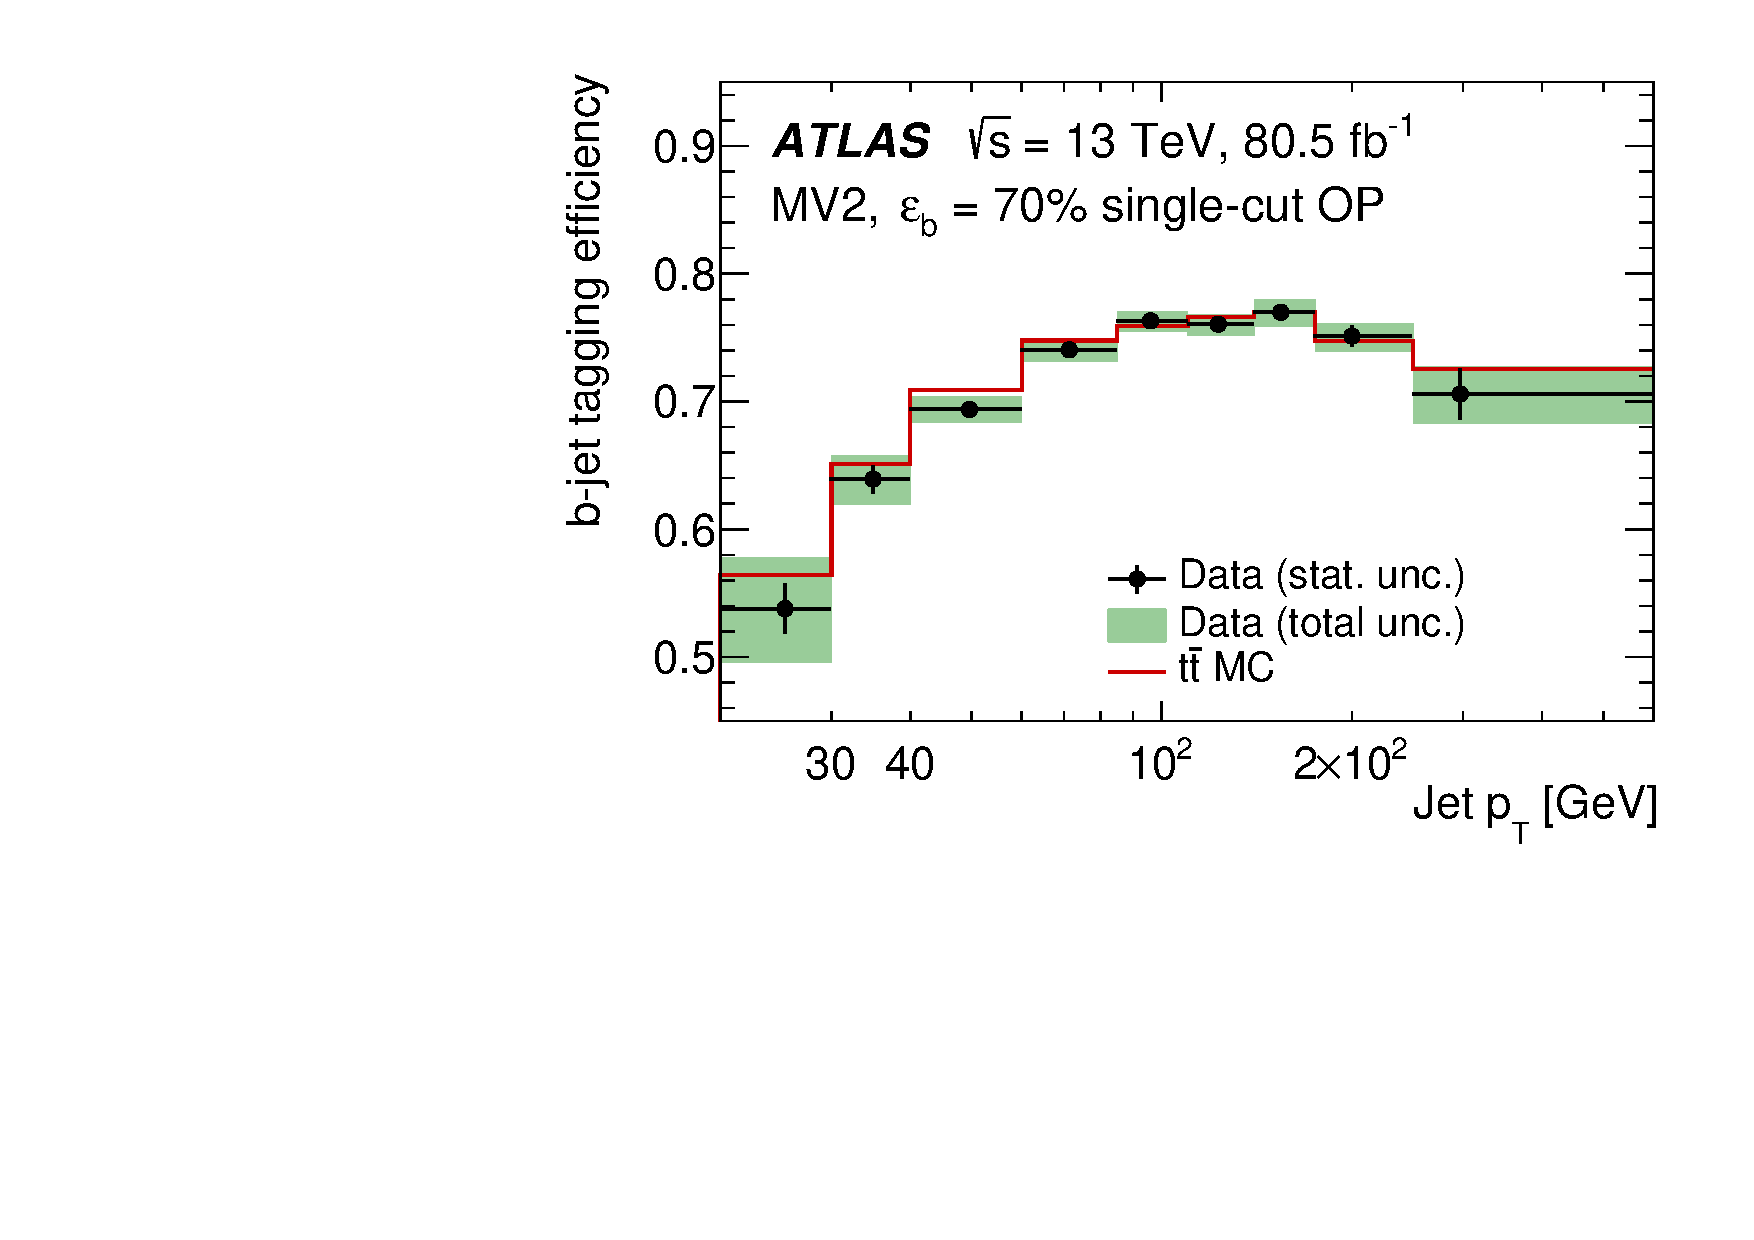
\includegraphics[width=0.48\textwidth]{figures/chapter3/ftag/ftag_eff_70_pt}
        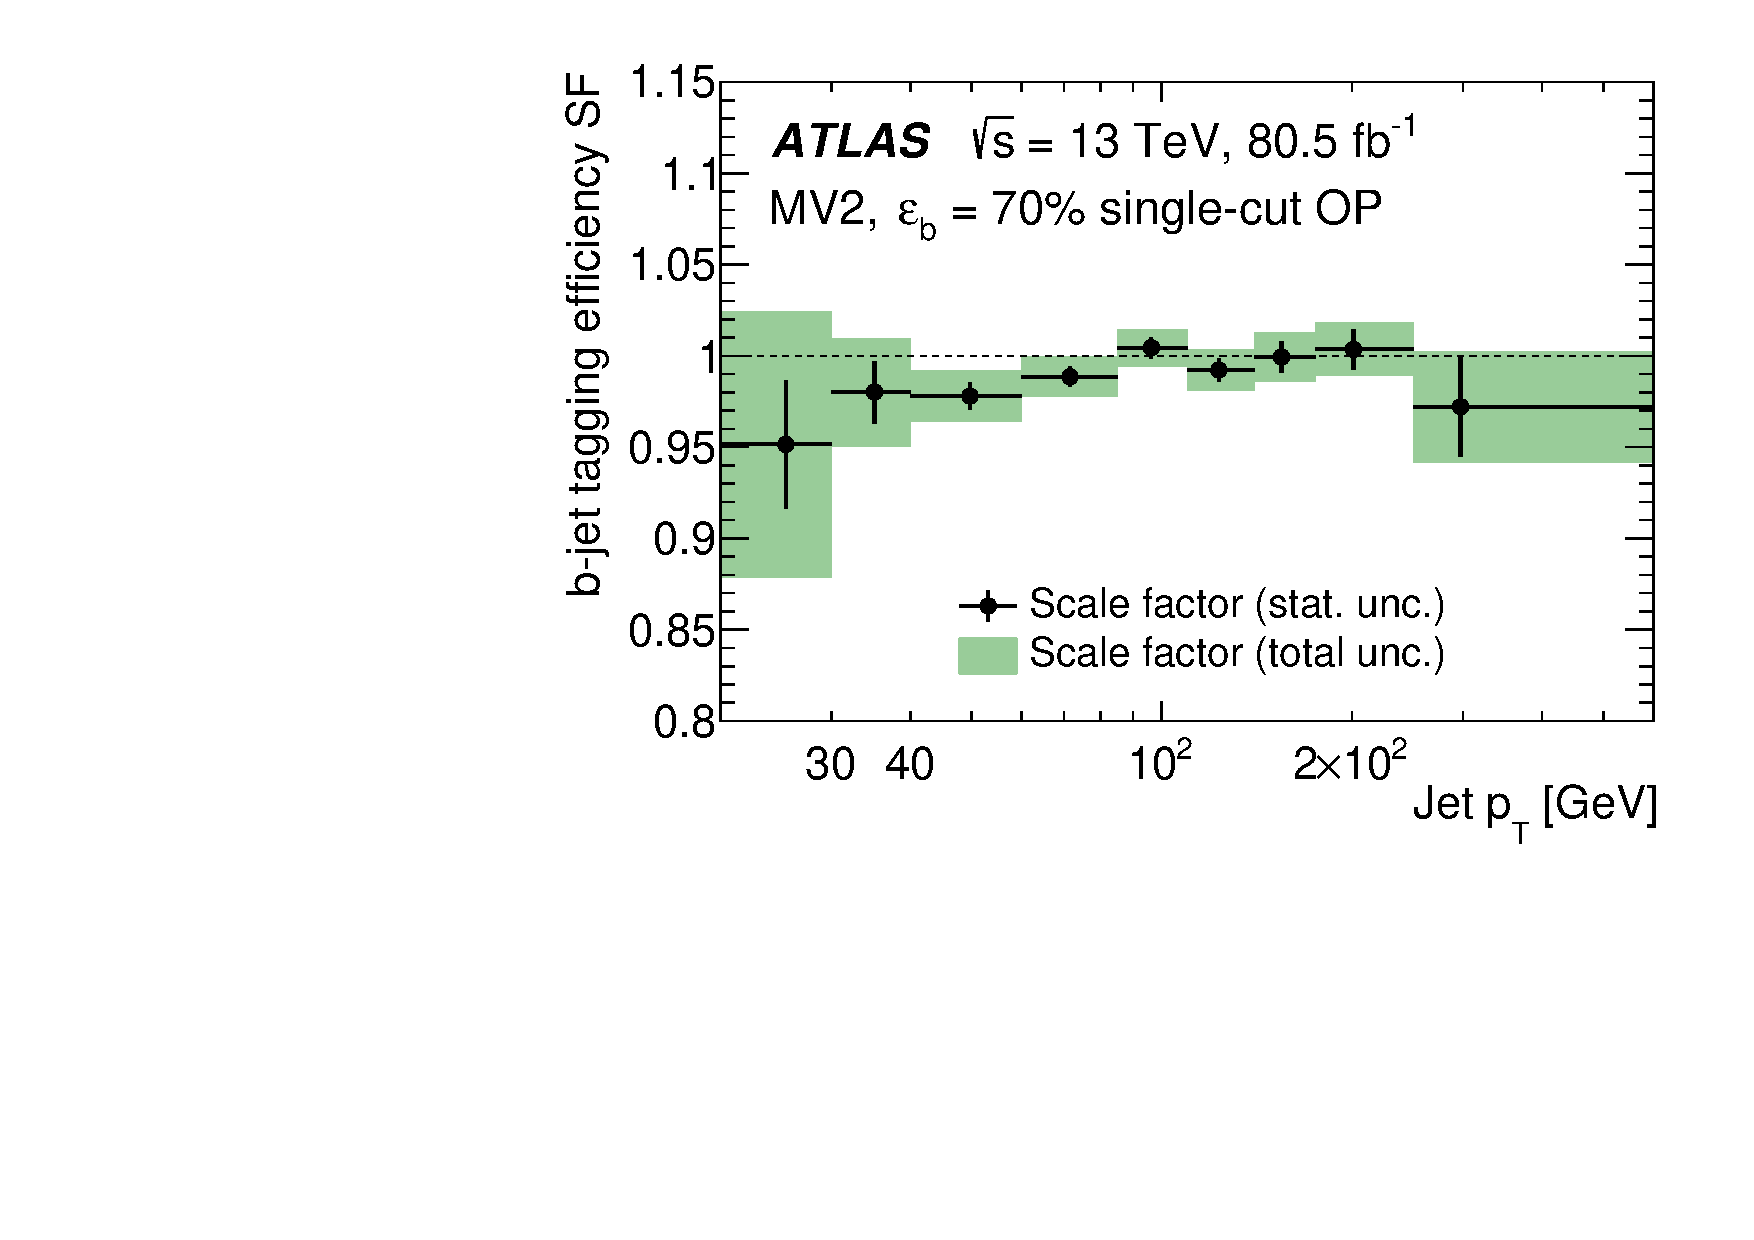
\includegraphics[width=0.48\textwidth]{figures/chapter3/ftag/ftag_sf_70_pt}
        \caption{
            \textit{Left}: $b$-jet tagging efficiency as a function of jet \pT~for the 70\% WP of the MV2 $b$-jet
                tagging algorithm in MC (top-quark pair production, in red) and data (black points).
                Efficiency values below and above 70\% occur, but the efficiency averaged over
                the full range shown is roughly 70\%. 
            \textit{Right}: $b$-jet tagging efficiency correction scale-factors for the 70\% WP of the MV2 $b$-jet
                tagging algorithm as a function of jet \pT~for the same
                samples as on the \textit{left}.
        }
        \label{fig:btag_eff_sf}
    \end{center}
\end{figure}



\FloatBarrier
